\documentclass[a4paper]{iutvexam}
% compile-latex options:--jobname controle20171218
% compile-latex options:--jobname correction20171218
\usepackage{textcomp,booktabs}
\usepackage{tikz}
\usetikzlibrary{calc}
\usepackage{listings}
\lstset{basicstyle=\ttfamily,
  showstringspaces=false,
  commentstyle=\itshape,
  keywordstyle=\bfseries,
  literate={á}{{\'a}}1 {ã}{{\~a}}1 {é}{{\'e}}1 
}

\title{Contrôle 2}
\date{18/12/2017}
\begin{document}
\conditions{ Vous disposez de 2 heures pour faire ce contrôle. Vous
  ferez \textbf{deux séries de question d'information} au choix,
  \textbf{deux séries de question de shell} au choix, et \textbf{une
    dernière au choix}. Les étudiants disposant d'un aménagement du
  temps, ne doivent traiter que deux de chaque série. Aucun document
  autorisé. Toute tentative de communication avec un voisin ou
  l'extérieur peut être sanctionnée. Toutes les réponses doivent être
  faites sur l'énoncé. La taille de la réponse attendue dépend de la
  taille allouée pour répondre. }
\begin{questions}
  \titledquestion{Information 1}

  Dans un processeur, la règle technologique (classique) suivante est
  toujours respectée:
  \begin{quote}
    les adresses d'une donnée (variable ou champ d'une variable de type
    \texttt{struct}) doivent toujours être un multiple de la taille de
    la variable si sa longueur en octets est moins qu'un mot-machine, et
    un multiple du mot-machine sinon.
  \end{quote}

  Dans le cas qui nous intéresse d'un processeur 32 bits, le mot-machine
  est un \texttt{int} de (évidemment) 32 bits, le \texttt{short int} est
  de 2 octets. Une adresse occupe un mot-machine aussi. L'ordinateur 32
  bits est un ordinateur \texttt{little endian} (les valeurs sur
  plusieurs octets sont stockées avec les poids faibles dans les petites
  adresses).

  Une structure \texttt{struct bidule} est définie par:

\begin{verbatim}
typedef struct bidule {  short int valeur; char longueur; char* adresse; }
\end{verbatim}

  Une variable \texttt{a} qui est un \texttt{struct bidule}, commence à l'adresse \texttt{0x8004} et est suivie d'une variable \texttt{b} de même type. La chaîne \texttt{c} est à l'adresse \texttt{0x8000}.

\begin{verbatim}
char *c="A0";
struct bidule a;
struct bidule b;
a.valeur=1023;
a.longueur=45;
a.nom=c;
\end{verbatim}

  Les schémas ci-dessous peuvent être plus grands que nécessaire. Ou pas.

  \begin{parts}
    \part[1] Représentez sur le schéma ci-dessous les cases mémoires occupées par la variable \texttt{a} et les cases mémoires occupées par la variable \texttt{b}.
    \part[1] Représentez sur le même schéma les cases mémoires occupées par chacun des champs des variables \texttt{a} et \texttt{b} (mettez le nom des champs dans les cases).

    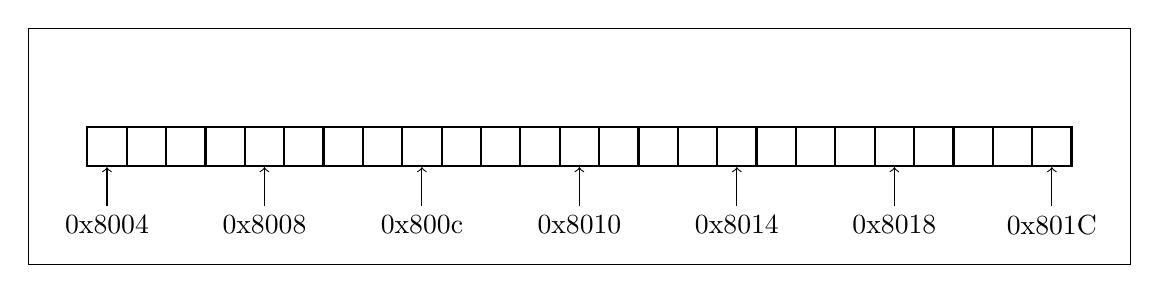
\begin{tikzpicture}
      \foreach \x in {4,5,...,28}{
        \node (a\x) [rectangle,draw=black,thick, minimum size=5mm] at (\x/2,0){};
      }
      \foreach \x/\y in {4/04,8/08,12/0c,16/10,20/14,24/18,28/1C}{
        \node (b\x) at ($ (a\x)+(0,-1) $) {0x80\y};
        \draw [->] (b\x) to (a\x);
      }
      \draw ($ (a4)+(-1,-1.5) $) rectangle ($ (a28)+(1,1.5) $);
    \end{tikzpicture}
    \part[1] Dans le schéma ci-dessous, représentez le contenu des cases mémoires en hexadécimal (ou en ASCII à votre choix) concernées par la chaîne \texttt{c}.
    \part[1] Dans le même schéma ci-dessous, représentez le contenu des cases mémoires en hexadécimal concernées par la variable \texttt{a}.

    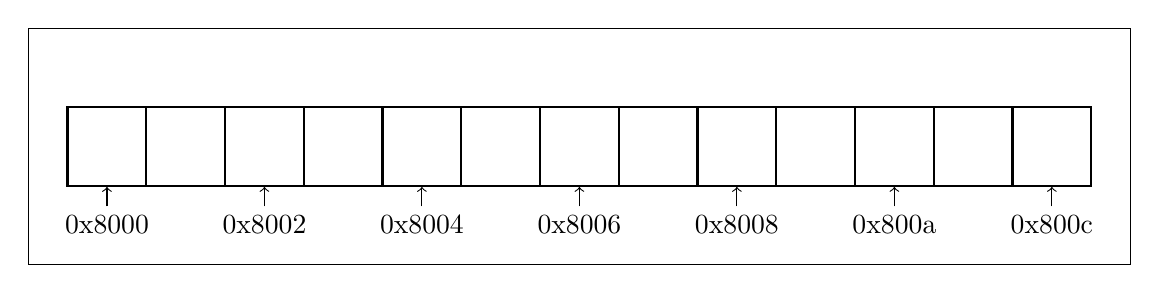
\begin{tikzpicture}
      \foreach \x in {0,1,...,12}{
        \node (a\x) [rectangle,draw=black,thick, minimum size=10mm] at (\x,0){};
      }
      \foreach \x/\y in {0/00,2/02,4/04,6/06,8/08,10/0a,12/0c}{
        \node (b\x) at ($ (a\x)+(0,-1) $) {0x80\y};
        \draw [->] (b\x) to (a\x);
      }
      \draw ($ (a0)+(-1,-1.5) $) rectangle ($ (a12)+(1,1.5) $);
    \end{tikzpicture}
  \end{parts}
  \newpage
  \titledquestion{Information 2}

  \begin{parts}
    \part[1] Expliquez deux façons possibles de coder la chaîne de caractère \texttt{"MÉROU"} dans divers environnements (il en existe au moins quatre, deux suffisent). Faites un schéma pour les deux.
    \begin{solutionorbox}[1in]%
      On peut soit faire varier l'encodage (ils n'ont pas besoin de connaître les codes exacts, juste expliquer et bien), soit le stockage (caractère nul terminal ou longueur puis données). UTF-8, ISO-latin d'un côté, caractère nul terminal ou valeur 5 en préfixe.
    \end{solutionorbox}

    \part[1] Un echantillon de son a été enregistré en stéréo pendant 10 secondes au format PCM: entête de 6 mots de 32 bits, avec codage des données à la suite de l'entête. La fréquence d'échantillonnage est de 8000 Hz, en \textmu-law (8 bits par échantillon) stéréo. Quelle est la taille du fichier final (tout compris) ? Décomposez le calcul.
    \begin{solutionordottedlines}[.25in]%
      8000*2*5 octets pour les données, 6*4 pour l'entête : 80024 octets.
    \end{solutionordottedlines}

    \part[1] Donnez un type de format le plus adapté pour ces quatre images:\\
    \begin{center}
      \begin{tabular}{c|c|c|c}
        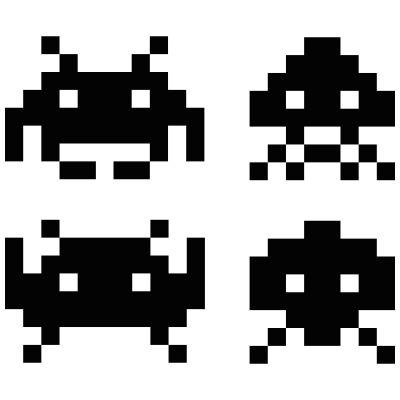
\includegraphics[width=.2\linewidth]{img/ctrl/invaders.jpg} &
                                                                      
\includegraphics[width=.2\linewidth]{img/ctrl/font.png} &
                                                                                                                                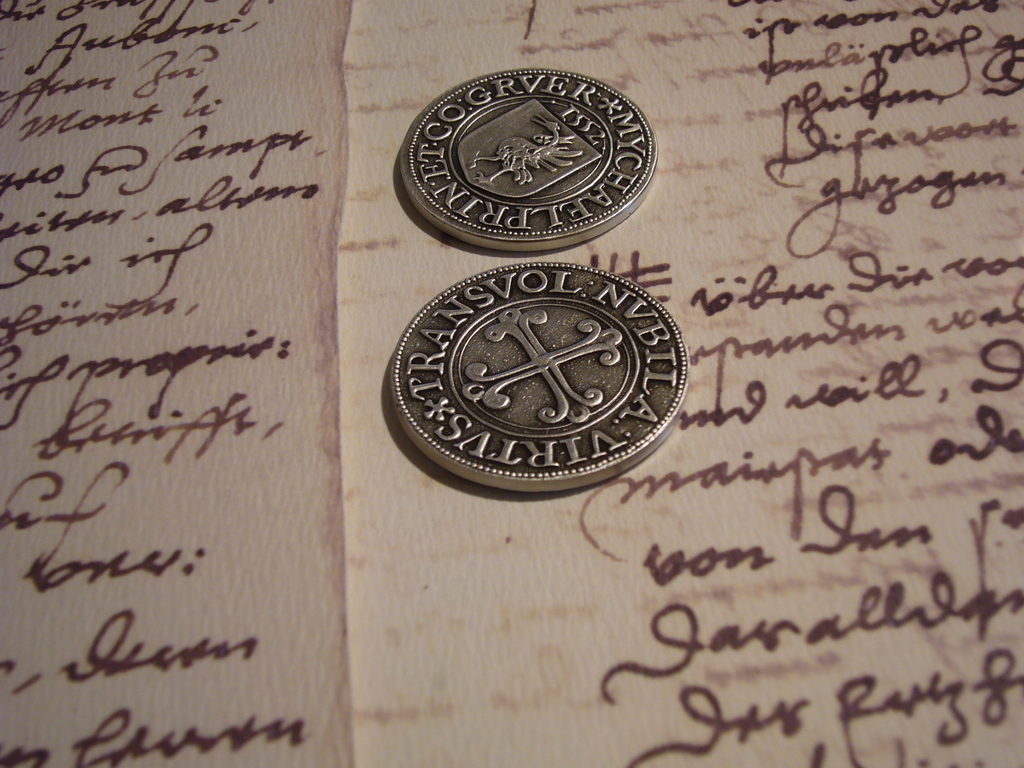
\includegraphics[width=.2\linewidth]{img/ctrl/fribourg-monnaie.jpg} &
                                                                                                                                                                                                      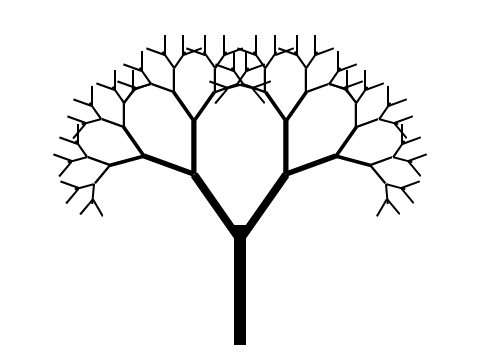
\includegraphics[width=.2\linewidth]{img/ctrl/fractaltree.png}
      \end{tabular}
    \end{center}
    \begin{solutionordottedlines}[.25in]%
      PNG, Vectoriel (ici c'est un PDF), JPG
    \end{solutionordottedlines}

    \part[1] Donnez une valeur plausible au «~format HTML~» pour les couleurs suivantes : bleu, jaune, violet foncé, rose très pâle.
    \begin{solutionordottedlines}[.25in]%
      0000FF, FFFF00, 400040, FFA0A0. On cherchera pour les deux derniers la bonne tendance plutôt qu'une valeur exacte: le violet c'est du rouge et du bleu en proportion à peu près égale, foncé donc pas trop lumineux ; le rose pâle, c'est du rouge mélangé avec du blanc.
    \end{solutionordottedlines}
  \end{parts}
  \newpage
  \titledquestion{Information 3}

  \begin{parts}
    \part[1] Une image est imprimée en hexachromie (six couleurs de
    base) avec un volume d'encre qui va de 5~p$\ell$ à 20~p$\ell$. La
    taille de la goutte est un nombre entier de picolitres. On peut
    déposer une goutte de chaque tous les 10 micromètres. Quel est le
    nombre de couleurs possible ? Quelle est la résolution de cette
    imprimante ? (considérez 1~in pour 2,54~cm pour les besoins de ce
    calcul de tête).
    \begin{solutionorbox}[1in]%
      16 niveaux par composante, donc $16^6$ couleurs en tout (ou
      $2^{24}$).  La résolution est de 100 points par millimètre, soit
      2540 points par pouce.
    \end{solutionorbox}

    \part[1] On veut stocker cette image sous forme d'une palette de
    couleur. On dénombre 65536 couleurs au maximum dans une des images
    de 1000 pixels sur 1000 pixels, soit $2^{16}$. Quel est la taille de
    la palette de couleur ? La taille des données de pixel ?
    \begin{solutionordottedlines}[.25in]%
      1000000 de pixels pour 2 octets chacun pour les données ($2.10^6$
      octets), et $2^{16}$ couleurs foit la taille trouvée ci-dessus,
      soit trois octets par élément.
    \end{solutionordottedlines}

    \part[1] On veut décrire des vaisseaux spatiaux de la flotte Zerg. Chacun a sa position dans l'espace par rapport au point de référence du vaisseau amiral, sa direction dans l'espace (vecteur vitesse), sa vitesse de rotation sur lui-même (sur les trois axes : roulis, tangage, lacet), le type (687 types de vaisseaux connus chez les Zergs), le nombre de canons (jusqu'à 148), l'équipage (quelques milliers au plus), et l'âge du capitaine (un Zerg vit au maximum 160 ans).
    Définissez une structure pour contenir le vaisseau, et donnez la taille en octets de chacun des éléments. Les données analogiques seront des \texttt{float}.
    \begin{solutionordottedlines}[3in]%
      
    \end{solutionordottedlines}

    \part[1] Dans un champ de bits sur 8 bits $a$: comment fait-on pour vérifier si le bit 0 est actif ou non. Décomposez
    l'opération. Comment fait-on pour forcer le bit 1 à 1 ? Et forcer le bit 3 à 0 ?
  \begin{solutionordottedlines}[.75in]%
    
  \end{solutionordottedlines}
\end{parts}

\newpage

\titledquestion{Système 1}

\begin{parts}

  \part[1] Expliquez en quelques mots ce qu'est un i-nœud. Précisez notamment la différence avec un chemin.
  \begin{solutionordottedlines}[.75in]%
    Un i-nœud est un bloc de données qui contient les informations sur
    un fichier (méta-données) ainsi qu'une localisation des données du
    fichier sur le disque. Un i-nœud peut être accédé par plusieurs chemins.
  \end{solutionordottedlines}


  \part[1] Un fichier \texttt{FICHE} est lisible, exécutable et
  modifiable par tout le monde. On veut le rendre lisible par tout son
  groupe, modifiable par soi uniquement, et interdit à tous les autres
  ; il n'est pas exécutables. Donnez les deux formes de commandes
  (symbolique et numérique) qui permettent de rendre ceci possible.
  \begin{solutionordottedlines}[.5in]%
    \verb|chmod o-rwx,g-wx,u-x FICHE| ou \verb|chmod 640 FICHE|
  \end{solutionordottedlines}

  \part[1] Expliquez brièvement le fonctionnement d'un processus au sein d'un système informatique (création, (in)activité, suppression).
  \begin{solutionordottedlines}[.75in]%
    création depuis un parent par fork, activité partagée par le système d'exploitation dans le temps, destruction après signalement au père.
  \end{solutionordottedlines}

  \part[1] Remplissez le tableau en indiquant pour chaque droit à
  quelle(s) action(s) il correspond dans le cas d'un fichier et d'un
  répertoire.
  \begin{center}
    \Large
    \begin{tabular}{p{4cm}cc}\toprule
      & pour un fichier &  pour un répertoire\\\midrule
      droit \texttt{r} & \hspace*{4cm} & \hspace*{4cm} \\
      droit \texttt{w} & \hspace*{4cm} & \hspace*{4cm} \\
      droit \texttt{x} & \hspace*{4cm} & \hspace*{4cm} \\\bottomrule
    \end{tabular}
  \end{center}
  \begin{solution}%
    lecture/modification/exécution et listing/suppression-création/traversée
  \end{solution}
\end{parts}

\titledquestion{Système 2}

Un répertoire \texttt{photos} contient des fichiers qui sont des photos
et des métadonnées sur les photos. Chaque photo est un fichier qui se
termine par l'extension \texttt{jpg}. Les métadonnées de chaque photo
ont le même nom terminé par \texttt{txt}. Les photos sont toutes
identifiées par une année et un numéro \texttt{ANNEE-IDENTIFIANT.txt}
(par exemple \texttt{2016-002348.jpg}). Chaque fichier de métadonnées
contient ainsi des lignes de données simples, comme par exemple
\texttt{auteur:Dubacq} ou \texttt{lieu:Paris} (une seule ligne
pour chaque clé maximum).

Vous êtes dans le répertoire qui contient \texttt{photos} (pas dans \texttt{photos}). Vous donnerez
vos réponses sous forme de scripts courts ou d'unilignes (scripts en
une ligne ; que vous pourriez taper directement dans le terminal,
donc).

Vous pouvez aussi écrire vos scripts en deux ou trois colonnes si
l'espace alloué n'est pas suffisant.

\begin{parts}
  \part[1] Déplacez toutes les photos d'une année (passée en paramètre numéro 1 du script), ainsi que leurs métadonnées, vers un répertoire \texttt{archivage} qui est à peut-être à créer.
  \begin{solutionordottedlines}[.75in]%
    \begin{lstlisting}[language=bash,caption={bash version}]
      #!/bin/bash
      mkdir -p archivage
      cp photos/$1-* archivage/ # $1 est le parametre
    \end{lstlisting}
  \end{solutionordottedlines}

  \newpage

  \part[1] Mettez dans une variable A le nombre de photos prises en 2016.
  \begin{solutionordottedlines}[1in]%
    \begin{lstlisting}[language=bash,caption={bash}]
      #!/bin/bash
      A=$(ls photos/2016*jpg|wc -l) # $A 
    \end{lstlisting}
  \end{solutionordottedlines}

  \part[1] Affichez le nombre de photos prises en 2016 en affichant
  \texttt{Nombre de photos en 2016: 257} (ou autre valeur). S'il n'y
  en pas, affichez \texttt{Pas de photos en 2016} (vous pouvez réutiliser la question ci-dessus).
  \begin{solutionordottedlines}[2in]%
    \begin{lstlisting}[language=bash,caption={bash}]
      #!/bin/bash
      A=$(ls photos/2016*jpg|wc -l)
      if [ $A -eq 0 ]; then
      echo "Pas de photos en 2016"
      else
      echo "Nombre de photos en 2016: $A" # $A plus haut
      fi
    \end{lstlisting}
  \end{solutionordottedlines}

  \part[1] Dans chaque fichier figure une ligne \texttt{qualité:} qui
  peut être \texttt{OK}, \texttt{KO}, ou \texttt{VOIR}. Dans un
  répertoire \texttt{partype}, faites autant de fichiers qu'il y a de
  qualités, et mettez dedans les noms des fichiers de la qualité
  correspondante (par exemple un fichier \texttt{KO} qui comportera
  les noms de tous les fichiers qui sont avec la qualité \texttt{KO}).

  \textbf{Rappel:} la commande \texttt{cut -d';' -f2} filtre chaque ligne en la
  découpant en morceaux séparés par les \texttt{;} présents dans la
  ligne et ne garde que le deuxième morceau. Exemple
  \texttt{toto;titi:tata;tutu} serait transformé en
  \texttt{titi:tata}. On peut évidemment changer le \texttt{2} et le
  \texttt{;}.

  \begin{solutionordottedlines}[2in]%
    \begin{lstlisting}[language=bash,caption={bash}]
      #!/bin/bash
      for i in photos/*; do
      TYPE=$(grep ^type: $i|cut -f2 -d:)
      echo $i >> partype/$TYPE
      done
    \end{lstlisting}
  \end{solutionordottedlines}

\end{parts}

\newpage
\titledquestion{Système 3}

\begin{parts}

  \part[1] Expliquez en quelques lignes ce que fait un processeur. Parlez notamment de son cycle vital.
  \begin{solutionordottedlines}[.75in]%
  \end{solutionordottedlines}


  \part[1] Faites un script simple qui dessine une pyramide de points à $n$ lignes, $n$ étant donné comme premier argument du script :
\begin{verbatim}
.
::.
::::.
::::::.
::::::::.
\end{verbatim}
  \begin{solutionordottedlines}[2in]%
    (double boucle)
  \end{solutionordottedlines}

  \part[1] Donnez au moins 4 commandes unix différentes qui ont une option. Expliquez ce que fait la commande habituellement, et ce que change l'option.
  \begin{solutionordottedlines}[2in]%
    ... à voir
  \end{solutionordottedlines}

  \part[1] Comment feriez-vous pour effacer un fichier dont le nom comporte un espace, comme par exemple \texttt{"Capture du 2017-12-18 11:00:14"} ? Et pour un nom qui comporte une apostrophe (\texttt{"Capture d'écran du 2017-12-18 11:00:14"}) ?
  \begin{solutionordottedlines}[2in]%
    rm avec des guillemets
  \end{solutionordottedlines}
\end{parts}

\end{questions}
\end{document}
